\documentclass[tikz, crop, border = {2pt 2pt 2pt 2pt}]{standalone}

\usepackage{physics}
\usepackage{concmath-otf}
\usetikzlibrary{decorations.pathreplacing}

\begin{document}
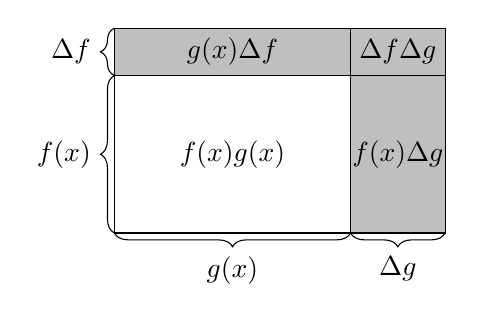
\begin{tikzpicture}
    \draw (0, 0) rectangle (3, 2) node[midway]{$f(x)g(x)$};
    \filldraw[fill = lightgray, draw = black] (3, 0) rectangle ++ (1.2, 2) node[midway]{$f(x)\Delta g$};
    \filldraw[fill = lightgray, draw = black] (0, 2) rectangle ++ (3, 0.6) node[midway]{$g(x) \Delta f$};
    \filldraw[fill = lightgray, draw = black] (3, 2) rectangle ++ (1.2, 0.6) node[midway]{$\Delta f\Delta g$};

    \draw[decorate, decoration = {brace, amplitude = 5pt, mirror}] (0, 0) -- (3, 0) node[midway, below = 5pt]{$g(x)$};
    \draw[decorate, decoration = {brace, amplitude = 5pt, mirror}] (3, 0) -- ++ (1.2, 0) node[midway, below = 5pt]{$\Delta g$};
    \draw[decorate, decoration = {brace, amplitude = 5pt}] (0, 0) -- ++ (0, 2) node[midway, left = 5pt]{$f(x)$};
    \draw[decorate, decoration = {brace, amplitude = 5pt}] (0, 2) -- ++ (0, 0.6) node[midway, left = 5pt]{$\Delta f$};
\end{tikzpicture}
\end{document}